\documentclass[a4paper, 12pt]{article}
\usepackage{cmap}
\usepackage[12pt]{extsizes}			
\usepackage{mathtext} 				
\usepackage[T2A]{fontenc}			
\usepackage[utf8]{inputenc}			
\usepackage[english,russian]{babel}
\usepackage{setspace}
\singlespacing
\usepackage{amsmath,amsfonts,amssymb,amsthm,mathtools}
\usepackage{fancyhdr}
\usepackage{soulutf8}
\usepackage{euscript}
\usepackage{mathrsfs}
\usepackage{listings}

\usepackage[colorlinks=true, urlcolor=blue, linkcolor=black]{hyperref}

\pagestyle{fancy}
\usepackage{indentfirst}
\usepackage[top=10mm]{geometry}
\rhead{}
\lhead{}
\renewcommand{\headrulewidth}{0mm}
\usepackage{tocloft}
\renewcommand{\cftsecleader}{\cftdotfill{\cftdotsep}}
\usepackage[dvipsnames]{xcolor}

\lstdefinestyle{mystyle}{ 
	keywordstyle=\color{OliveGreen},
	numberstyle=\tiny\color{Gray},
	stringstyle=\color{BurntOrange},
	basicstyle=\ttfamily\footnotesize,
	breakatwhitespace=false,         
	breaklines=true,                 
	captionpos=b,                    
	keepspaces=true,                 
	numbers=left,                    
	numbersep=5pt,                  
	showspaces=false,                
	showstringspaces=false,
	showtabs=false,                  
	tabsize=2
}

\lstset{style=mystyle}

\begin{document}
\thispagestyle{empty}
\begin{center}
    Московский авиационный институт

    (Национальный исследовательский университет)

    Факультет "Информационные технологии и прикладная математика"

    Кафедра "Вычислительная математика и программирование"

\end{center}
\vspace{40ex}
\begin{center}
    \textbf{\large{Лабораторная работа №2 по курсу\linebreak \textquotedblleft Операционные системы\textquotedblright}}
\end{center}
\vspace{35ex}
\begin{flushright}
    \textit{Студент: } Кочкожаров Иван Вячеславович

    \vspace{2ex}
    \textit{Группа: } М8О-208Б-22

    \vspace{2ex}
    \textit{Преподаватель: } Миронов Евгений Сергеевич

    \vspace{2ex}
    \textit{Вариант: } 13

    \vspace{2ex}
    \textit{Оценка: } \underline{\quad\quad\quad\quad\quad\quad}

    \vspace{2ex}
    \textit{Дата: } \underline{\quad\quad\quad\quad\quad\quad}

    \vspace{2ex}
    \textit{Подпись: } \underline{\quad\quad\quad\quad\quad\quad}

\end{flushright}

\vspace{5ex}

\begin{vfill}
    \begin{center}
        Москва, 2023
    \end{center}
\end{vfill}
\newpage

\begingroup
\color{black}
\tableofcontents\newpage
\endgroup

\section{Репозиторий}
\href{https://github.com/kochkozharov/os-labs}{https://github.com/kochkozharov/os-labs}

\section{Цель работы}
Приобретение практических навыков в:
\begin{itemize}
    \item Управлении потоками в ОС
    \item Обеспечении синхронизации между потоками
\end{itemize}

\section{Задание}
Составить программу на языке Си, обрабатывающую данные в многопоточном режиме. При обработки использовать стандартные средства создания потоков операционной системы (Windows/Unix). Ограничение максимального количества потоков, работающих в один момент времени, должно быть задано ключом запуска вашей программы.

\section{Описание работы программы}
Необходимо было написать программу для наложения матрицы свертки на изображение. Изображение разбивается на массивы равной длинны и каждый процесс применяет матрицу свертки к своему участку. После каждой итерации происходит синхронизация по барьеру во избежание проблем с граничными пикселями
В ходе выполнения лабораторной работы использованы следующие системные вызовы:
\begin{itemize}
    \item pthread\_create() - создание потока
    \item pthread\_join() - ожидание завершения потока
\end{itemize}

\newpage

\section{Исходный код}
blur.c
\begin{lstlisting}[language=C++]
    #include "blur.h"

    #include <assert.h>
    #include <pthread.h>
    #include <stdio.h>
    #include <stdlib.h>
    #include <string.h>
    #include <unistd.h>
    
    static void Convolution(const Image* img, size_t idx, const Kernel* ker,
                            uc (*out)[]) {
        uc(*imgMat)[img->width] = img->matrix;
        const int(*kerMat)[ker->order] = ker->matrix;
        uc(*outMat)[img->width] = out;
        const size_t absI = idx / img->width * img->channels;
        const size_t absJ = idx % img->width * img->channels;
        size_t sum[MAX_CHANNELS] = {0};
    
        for (int i = -(ker->order / 2); i <= ker->order / 2; ++i) {
            for (int j = -ker->order / 2; j <= ker->order / 2; ++j) {
                const int kerI = i + ker->order / 2;
                const int kerJ = j + ker->order / 2;
    
                size_t imgI;
                if (i < 0 && (size_t)-i * img->channels > absI) {
                    imgI = 0;
                } else {
                    imgI = (size_t)i * img->channels + absI;
                    if (imgI > (img->height - 1) * img->channels) {
                        imgI = (img->height - 1) * img->channels;
                    }
                }
    
                size_t imgJ;
                if (j < 0 && (size_t)-j * img->channels > absJ) {
                    imgJ = 0;
                } else {
                    imgJ = (size_t)j * img->channels + absJ;
                    if (imgJ > (img->width - 1) * img->channels) {
                        imgJ = (img->width - 1) * img->channels;
                    }
                }
    
                int coef = kerMat[kerI][kerJ];
                for (int k = 0; k < img->channels; ++k) {
                    sum[k] += (size_t)coef * imgMat[imgI][imgJ + k];
                }
            }
        }
        for (int k = 0; k < img->channels; ++k) {
            outMat[absI][absJ + k] = sum[k] / ker->divCoef;
        }
    }
    static void* ChunkConvolution(void* ptr) {
        ThreadArgs* arg = ptr;
        uc(*buf)[] = arg->buf;
        for (int iteration = 0; iteration < arg->times; ++iteration) {
            for (size_t i = arg->begin; i < arg->end; ++i) {
                Convolution(arg->img, i, arg->ker, buf);
            }
            int status = pthread_barrier_wait(arg->barrier);
            if (status != 0 && status != PTHREAD_BARRIER_SERIAL_THREAD) {
                perror("pthread_barrier_wait");
                exit(EXIT_FAILURE);
            }
            uc(*temp)[] = arg->img->matrix;
            arg->img->matrix = buf;
            buf = temp;
        }
        return NULL;
    }
    
    const uc* ApplyKernel(Image* img, const Kernel* kernel, int k, uc (*buffer)[], unsigned long threadsNum) {
        assert(kernel->order % 2 == 1 && img->channels <= MAX_CHANNELS);
        int status;
        size_t matrixSize = img->height * img->width;
        pthread_barrier_t barrier;
        status = pthread_barrier_init(&barrier, NULL, threadsNum);
        if (status != 0) {
            perror("pthread_barrier_init");
            exit(status);
        }
    
        pthread_t *threads=malloc(threadsNum*sizeof(pthread_t));
        ThreadArgs *args=malloc(threadsNum*sizeof(ThreadArgs));
        size_t pixelsPerThread = matrixSize / threadsNum;
    
        for (unsigned long i = 0; i < threadsNum; ++i) {
            size_t begin = i * pixelsPerThread;
            size_t end = i == threadsNum - 1 ? matrixSize : begin + pixelsPerThread;
            args[i] = (ThreadArgs){.img = img,
                                   .begin = begin,
                                   .end = end,
                                   .ker = kernel,
                                   .buf = buffer,
                                   .times = k,
                                   .barrier = &barrier};
            status = pthread_create(&threads[i], NULL, ChunkConvolution, &args[i]);
            if (status != 0) {
                perror("pthread_create");
                exit(status);
            }
        }
        for (unsigned long i = 0; i < threadsNum; ++i) {
            pthread_join(threads[i], NULL);
        }
    
        pthread_barrier_destroy(&barrier);
        free(threads);
        free(args);
        return (uc*)(k % 2 == 1 ? buffer : img->matrix);
    }
\end{lstlisting}

main.c
\begin{lstlisting}[language=C++]
    #include <getopt.h>
#define STB_IMAGE_IMPLEMENTATION
#include <stb/stb_image.h>
#define STB_IMAGE_WRITE_IMPLEMENTATION
#include <stb/stb_image_write.h>
#include <time.h>

#include "blur.h"

//#define TEST

typedef enum { gauss, box } TFilter;

static const Kernel GAUSSIAN5 = {
    .matrix =
        (const int[5][5]){
            {1, 4, 6, 4, 1},
            {4, 16, 24, 16, 4},
            {6, 24, 36, 24, 6},
            {4, 16, 24, 16, 4},
            {1, 4, 6, 4, 1},
        },
    .order = 5,
    .divCoef = 256,
};

static const Kernel BOX3 = {
    .matrix =
        (const int[3][3]){
            {1, 1, 1},
            {1, 1, 1},
            {1, 1, 1},
        },
    .order = 3,
    .divCoef = 9,
};

int main(int argc, char *argv[]) {
#ifdef TEST
    (void)BOX3;
    if (argc < 2) {
        fprintf(stderr,
                "Usage: blur INPUT_FNAME\n");
        exit(EXIT_SUCCESS);
    }
#else
    if (argc < 3 || strcmp(argv[1], "--help") == 0) {
        fprintf(stderr,
                "Usage: blur INPUT_FNAME OUTPUT_FNAME -f FILTER -k K (apply "
                "filter FILTER K times)\n");
        exit(EXIT_SUCCESS);
    }

    long times = 1;
    unsigned long threadsNum = DEF_THREAD_NUM;
    TFilter filter = gauss;
    const char *filterName;
    for (int opt; opt = getopt(argc, argv, "f:k:t:r"), opt != -1;) {
        switch (opt) {
            case '?':
                perror("getopt");
                exit(EXIT_FAILURE);
            case 'f':
                if (strcmp(optarg, "box") == 0) {
                    filter = box;
                }
                break;
            case 'k': {
                char *end;
                times = strtol(optarg, &end, 10);
                break;
            }
            case 't': {
                char *end;
                threadsNum = strtol(optarg, &end, 10);
                break;
            }
        }
    }
#endif

    int width;
    int height;
    int channels;

#ifndef TEST
    stbi_uc *img = stbi_load(argv[argc - 2], &width, &height, &channels, 0);
#else
    stbi_uc *img = stbi_load(argv[1], &width, &height, &channels, 0);
#endif

    if (img == NULL) {
        perror("stbi_load");
        exit(EXIT_FAILURE);
    }
    printf("Loaded. x: %dpx y: %dpx channels: %d.\n", width, height, channels);

    size_t imgSize = (size_t)width * height * channels;
    stbi_uc *buf = malloc(imgSize);
    if (!buf) {
        perror("malloc");
        exit(EXIT_FAILURE);
    }

    const Kernel *ker = &GAUSSIAN5;

#ifdef TEST
    const stbi_uc *weakPtr;
    for (int threads = 1; threads < 21; ++threads) {
        printf("Applying gaussian blur 20 times on %d threads\n", threads);
#else
    if (filter == box) {
        ker = &BOX3;
        filterName = "box";
    } else {
        filterName = "gaussian";
    }
    printf("Applying %s blur %ld times on %ld threads\n", filterName, times,
           threadsNum);
#endif

        struct timespec start;
        struct timespec finish;
        clock_gettime(CLOCK_MONOTONIC, &start);
#ifdef TEST
        weakPtr = ApplyKernel(&(Image){.matrix = (stbi_uc(*)[])img,
                                       .width = width,
                                       .height = height,
                                       .channels = channels},
                              ker, 20, (stbi_uc(*)[])buf, threads);
#else
    const stbi_uc *weakPtr =
        ApplyKernel(&(Image){.matrix = (stbi_uc(*)[])img,
                             .width = width,
                             .height = height,
                             .channels = channels},
                    ker, (int)times, (stbi_uc(*)[])buf, threadsNum);
#endif
        clock_gettime(CLOCK_MONOTONIC, &finish);
        double elapsed;
        elapsed = (finish.tv_sec - start.tv_sec);
        elapsed += (finish.tv_nsec - start.tv_nsec) / 1.0E9;
        printf("Function took %fs to execute\n", elapsed);

#ifdef TEST
    }
    printf("Test end\n");
#endif

#ifdef TEST
    int status =
        stbi_write_jpg("result.jpg", width, height, channels, weakPtr, 100);
#else
    int status =
        stbi_write_jpg(argv[argc - 1], width, height, channels, weakPtr, 100);
#endif

    if (status == 1) {
        printf("Successfully written %zu bytes\n",
               (size_t)width * height * channels);
    } else {
        perror("stbi_write_jpg");
        exit(EXIT_FAILURE);
    }

    stbi_image_free(img);
    free(buf);
    return 0;
}
\end{lstlisting}

\newpage
\section{Тесты}
\begin{lstlisting}[language=C++]
#include <gtest/gtest.h>

extern "C" {
#include "blur.h"
}

TEST(SecondLabTests, SimpleTest) {
    const size_t width = 4;
    const size_t height = 2;
    const uc example[height][width] = {{1, 2, 3, 4}, {1, 2, 3, 4}};
    uc imgMat[height][width];
    memcpy(imgMat, example, width * height);
    Image img = {reinterpret_cast<uc(*)[]>(imgMat), width, height, 1};
    const int kerMat[3][3] = {1, 1, 1, 1, 1, 1, 1, 1, 1};
    const Kernel ker = {reinterpret_cast<const int(*)[]>(kerMat), 3, 9};
    uc buf[height][width];
    const uc excpectedRes[height][width] = {{1, 2, 3, 3}, {1, 2, 3, 3}};
    const uc *weakPtr = ApplyKernel(&img, &ker, 1, reinterpret_cast<uc(*)[]>(buf), 1);
    for (unsigned int i = 0; i < height; ++i) {
        for (unsigned int j = 0; j < width; ++j) {
            uc c = *(weakPtr + i * width + j);
            uc rc = excpectedRes[i][j];
            EXPECT_EQ(c, rc);
        }
    }
    memcpy(imgMat, example, width * height);
    img.matrix = reinterpret_cast<uc(*)[]>(imgMat);
    weakPtr = ApplyKernel(&img, &ker, 1, reinterpret_cast<uc(*)[]>(buf), 4);
    for (unsigned int i = 0; i < height; ++i) {
        for (unsigned int j = 0; j < width; ++j) {
            uc c = *(weakPtr + i * width + j);
            uc rc = excpectedRes[i][j];
            EXPECT_EQ(c, rc);
        }
    }
}
\end{lstlisting}

\newpage
\section{Консоль}
\begin{verbatim}
ivan@asus-vivobook ~/c/o/b/lab2 (reports)> ./blur 1024px-Lenna.png result.jpg -k 10
Loaded. x: 1024px y: 1024px channels: 3.
Applying gaussian blur 10 times on 12 threads
Function took 0.635936s to execute
Successfully written 3145728 bytes
\end{verbatim}


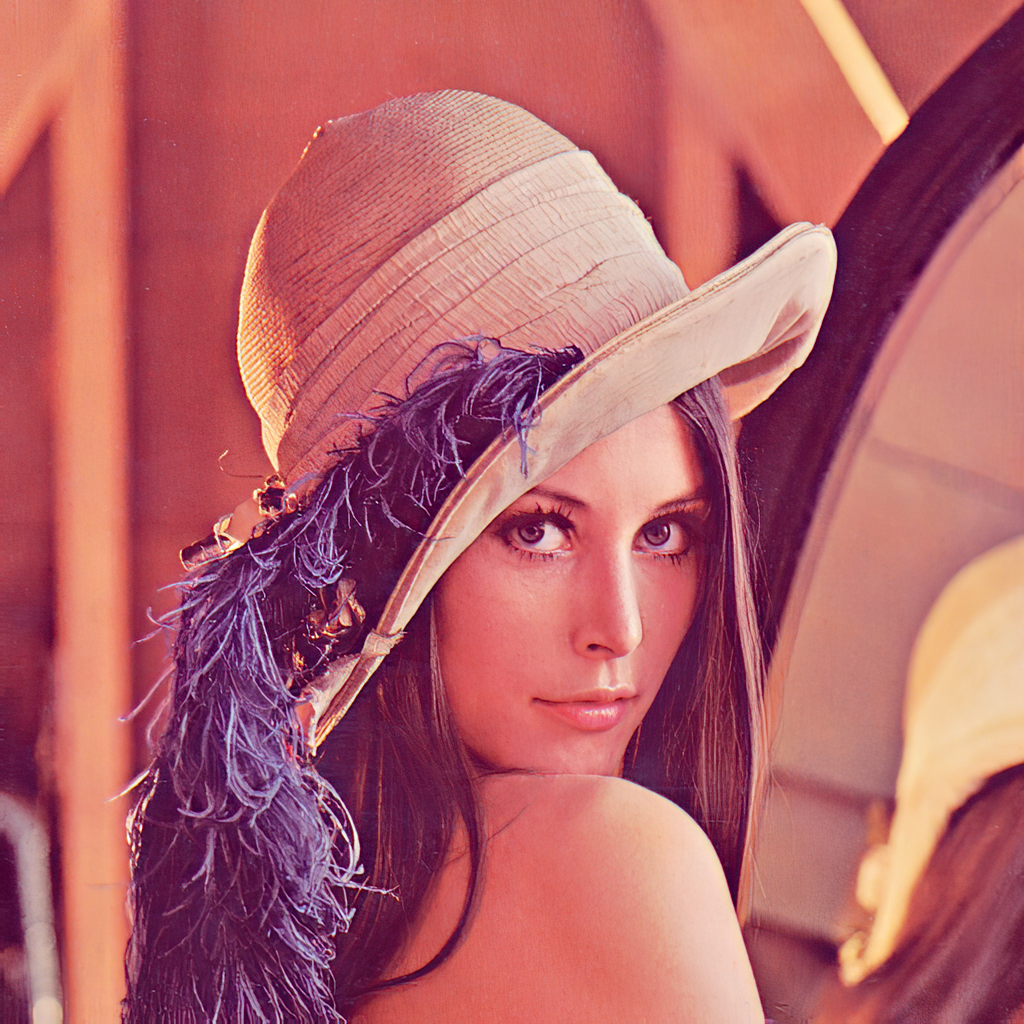
\includegraphics[width=0.5\linewidth]{lenna.png}

\includegraphics[width=0.5\linewidth]{lenna_blur.png}







\newpage
\section{Запуск тестов}
\begin{verbatim}
Running main() from /var/tmp/portage/dev-cpp/gtest-1.13.0/work/googletest-1.13.0/googletest/src/gtest_main.cc
[==========] Running 1 test from 1 test suite.
[----------] Global test environment set-up.
[----------] 1 test from SecondLabTests
[ RUN      ] SecondLabTests.SimpleTest
[       OK ] SecondLabTests.SimpleTest (1 ms)
[----------] 1 test from SecondLabTests (1 ms total)

[----------] Global test environment tear-down
[==========] 1 test from 1 test suite ran. (1 ms total)
[  PASSED  ] 1 test.
\end{verbatim}
%
Ускорение:
\begin{equation}
    S_4 = \cfrac{T_1}{T_4} < 4
\end{equation}

\begin{equation}
    S_4 = \cfrac{7.323169}{1.848535} = 3.96 < 4
\end{equation}

Эффективность:
\begin{equation}
    X_4 = \cfrac{S_4}{4} < 1
\end{equation}

\begin{equation}
    X_4 = \cfrac{3.96}{4} = 0.99 < 1
\end{equation}

\newpage
\section{Выводы}

В результате выполнения данной лабораторной работы была написана программа на языке С для наложения матричных фильтров на изображения, обрабатывающая данные в многопоточном режиме. Приобретены практические навыки в управлении потоками в ОС и обеспечении синхронизации между потоками.
\end{document}